% 2019-05-22 11:20--11:40
% 7. Leipziger Semantic Web Tag, English presentation about the SNIK project and ontology.
% 15 minutes presentation, 5 minutes for questions.

%\documentclass[aspectratio=43]{beamer}
%\documentclass[aspectratio=169]{beamer}
\documentclass[aspectratio=1610,12pt]{beamer}
%\usepackage{pgfpages}
%\setbeameroption{show notes}
%\setbeameroption{show notes on second screen=right}
\usepackage[ngerman]{babel}
\usepackage{booktabs} % fancy tables
\usepackage{tabulary} % tables with auto column length 
\usepackage{hyperref}
\usepackage{siunitx}

\usetheme{imise2}
\author{Konrad Höffner}%, Institute for Medical Informatics, Statistics and Epidemiology}
%\title{The SNIK Ontology of Information Management in Hospitals}
\title{\Large SNIK -- Ein Semantisches Netz des Informationsmanagements im Krankenhaus}
\subtitle{}
\date{5.\,12.\,2019, IWIMI 2019}
\def\address{Härtelstraße 16-18, 04107 Leipzig, Raum 227}
\def\email{konrad.hoeffner@imise.uni-leipzig.de} 
\def\telephone{+49 341 97 16322}

% TODO: Use SNIK Graph as title slide, get audience attention right away

\newcommand{\imageslide}[4][]
{
\newgeometry{margin=0cm,top=1em}
\begin{frame}[plain]{~~~~#2}
\vspace{0.2em}
\centering\includegraphics[width=1.0\textwidth,height=0.95\textheight,keepaspectratio]{#3}
\\#1
\note{#4}
\end{frame}
\restoregeometry
}

\begin{document}


{
\setbeamertemplate{background canvas}%
{
 \vbox to \paperheight{\vfil\hbox to \paperwidth{%
 \hfil \includegraphics[width=\paperwidth,height=\paperheight,keepaspectratio]{img/snik-graph.png} \hfil}
 }
}
\begin{frame}
\titlepage
\end{frame}
}

\newgeometry{margin=0cm,top=1em}
\begin{frame}[plain]{~~~~Domäne}
% Information Management in Hospitals is a core topic for students of medical computer science.
% Unfortunately, there are many different views of the domain, whose relationship is often unclear, and the terminology is full of synonyms and homonyms.
% So this domain is difficult to learn for students. 
\centering\includegraphics[height=0.77\textheight,keepaspectratio]{img/book-bb.jpg}
\centering\includegraphics[height=0.77\textheight,keepaspectratio]{img/book-ob.jpg}
\centering\includegraphics[height=0.77\textheight,keepaspectratio]{img/book-he.jpg}
\end{frame}
\restoregeometry
\imageslide{Vokabular}{img/wordcloud-ob.png}{}{}

\imageslide{Synonyme}{img/wordcloud-synonym.png}{}{}
% Überleitung ?
\imageslide{Metamodell}{img/metamodel9s.pdf}{}{}
% Welche Beispiele? für begriffe und für relationen
\imageslide{Modellierungsbeispiel}{img/bb-cio.pdf}{}{}

\newgeometry{margin=0cm,top=1em}
\begin{frame}[plain]{~~~~Transformation}
\centering\includegraphics[height=0.21\textheight,keepaspectratio]{img/book-bb.jpg}
\centering\includegraphics[height=0.21\textheight,keepaspectratio]{img/book-ob.jpg}
\centering\includegraphics[height=0.21\textheight,keepaspectratio]{img/book-he.jpg}
\centering\includegraphics[width=0.7\textwidth,keepaspectratio]{img/5star.png}
\end{frame}
\restoregeometry

\imageslide{Lifecycle}{cycle.pdf}

\imageslide{Setup}{img/architecture.png}

%\newgeometry{margin=0cm,top=1em}

\imageslide{Speichern und Abfragen -- Virtuoso SPARQL Endpoint}{img/virtuoso.png}{}{}

\begin{frame}{Speichern und Abfragen -- Virtuoso SPARQL Endpoint}
\begin{itemize}
\item Kernservice, auf dem fast alle anderen aufbauen 
\item SPARQL ist defacto-Standard-Abfragespache für Linked Data
\item Experten können selbst abfragen stellen, andere greifen auf Services zu
\item analog zu relationaler Datenbank
\end{itemize}
\end{frame}

\imageslide{Autorenwerkzeug OntoWiki}{img/ontowiki.png}{}{}
\imageslide{Interlinks mit LIMES}{img/limes.png}{}{}
\imageslide{Browsing}{img/lodview.png}{}{}

\imageslide{SNIK Qualitätscheck}{img/qualitycheck.png}{}{}

\imageslide{Suche \& Exploration: SNIK Graph}{img/snik-graph-full.png}{}{}

% Classes as Nodes
% Triples as Edges
% Force Directed Layout
% Color Coding Based on Source
\imageslide{SNIK Graph---Ontologievisualisierung}{img/graph-entitytype.png}{}{}
\imageslide{SNIK-Graph---Begriffsnutzung}{img/roleuse-wide.png}{}{}

\imageslide{SNIK-Graph---Spiderworm}{img/spider.png}{}{}
\imageslide{SNIK-Graph---Exploration}{img/snik-graph-star.png}{}{}


\textit{Krankenhaus-Informations-System} ist ein Homonym:
1. Die Menge an Hardware, Software und deren Benutzer 
2. Ein spezielles Software-Produkt im Krankenhaus

Synonyme: Chief Information Officer (CIO) --- IT Manager

\begin{itemize}
\item large domain
\item different textbooks and frameworks with different views
\item different names for the same concept (synonyms)
\item same name for different concepts  (homonyms)
\item unclear relationship between sources
\end{itemize}

select *
{
 ?s a owl:Class.
 ?s rdfs:label ?l.
 ?s skos:altLabel ?al.
 filter(langMatches(lang(?l),"en"))
 filter(langMatches(lang(?al),"en"))
}

\begin{frame}{Projektziele}
\begin{enumerate}
\item create a modular ontology of Information Management in Hospitals:
\begin{itemize}
\item develop a core vocabulary (meta model)
\item transform textbooks to subontologies 
\end{itemize}
\item manage Linked Data Lifecycle 
\item create teaching tools
\item offer low-threshold self-learning tools to students
\end{enumerate}
\end{frame}

%\section{Ontology Creation}


\newgeometry{margin=0cm,top=1em}
\begin{frame}[plain]{~~~~Example}
~\\~\\
\begin{itemize}
\item excerpt of \emph{Health Information Systems}, A. Winter et al.
\item CIO is responsible for different functions and entity types
\item functions read information from or write it to the Strategic Information Management Plan
\end{itemize}
~\\~\\
\centering\includegraphics[width=\textwidth,keepaspectratio]{img/snik-graph-cio.png}
\end{frame}
\restoregeometry


\begin{frame}{Transformation Challenges}
\begin{itemize}
\item manual, time-consuming extraction
\item not all extractors have Semantic Web skills 
\begin{itemize}
\item table as intermediate step
\item "media discontinuity", loss of information
\item inference of OWL restrictions from limited data 
\end{itemize}
\item modelling as classes vs. individuals
\item detailed ontology modelling vs. large amounts of instances 
\end{itemize}
\end{frame}

\newgeometry{margin=0cm,top=1em}
\begin{frame}[plain]{~~~~Applications}
% SNIK stands for Semantic Network of Information Management in Hospitals (German "Krankenhaus") and tries to unify those views.
\centering\includegraphics[height=0.95\textheight,keepaspectratio]{img/snik-graph.png}
\end{frame}
\restoregeometry

%\imageslide{RDF Browser LodView}{img/lodview.png}
\imageslide[\url{http://www.snik.eu} \url{http://5stardata.info}]{SNIK Projekt}{img/5star.png}
{
\begin{itemize}
\item kurze Einführung SNIK-Projekt
\item offene Bereitstellung von computerverarbeitbaren Fakten des Informationsmanagements im Krankenhaus aus Lehrbüchern
\item Nutzen maximieren: 5 Sterne Schema für offene Daten von Tim Berners-Lee
\end{itemize}

\begin{enumerate}
\item Rechtssicherheit für Benutzer durch offene Datenlizenz. PDFs der Bücher dürfen allerdings nicht online gestellt werden. Nur wenn jemand fragt:
\begin{itemize}
\item CC BY-NC-SA 4.0 Lizenz (Creative Commons Attribution-NonCommercial-ShareAlike).
\item Erlaubt: Teilen, Adaptieren
\item Bedingungen: Attribution, Nichtkommerziell, gleiche Lizenz für Derivate. Für eine offene Lizenz recht restriktiv, sind aber für andere Optionen offen
\end{itemize}
\item Strukturiertes Format: Lesen der Bücher und manuelles modellieren der Fakten in Tabellen, sehr zeitaufwändig 
\item Stufe 3 trivial: speichern in offenem Format, in unserem Fall CSV
\item Konvertierung der Tabelle zu einer Ontologie mittels Tarql scripts, viel Vorarbeit in Tabellen 
\item Interlinks zwischen Büchern automatisch erstellt durch LIMES
\end{enumerate}
}

\begin{frame}{Einsatz}
\centering
\begin{tabular}{ll}
\toprule
\textbf{Ziel}	&\textbf{Zielgruppe}\\
\midrule
Lehre			&Lehrer und Studenten\\ 
Datenintegration	&Krankenhausleitung, CIO\\
Formalisierung		&Domänenexperten, Ontologen\\
\bottomrule
\end{tabular}
\note{
\begin{itemize}
\item benötigte Tools hängen von Zielen und Zielgruppen ab 
\item Lehre: Vermittlung des Fachwissens an Studenten. Für Vorteil gegenüber/zusätzlich zu Lesen der Bücher: kein Vorwissen, schnelle, simple und intuitive Wissensvermittlung.
\item Datenintegration: Ontologie kann als Vokabular von verschiedenen Anwendungen benutzt werden
\item Verbesserung des durch Studenten extrahierten formalisierten Fachwissens durch Ontologen und Domänenexperten
\end{itemize}
}
\end{frame}

%\imageslide[\url{https://github.com/IMISE/snik-ontology}]{Ausgangspunkt: RDF Dump}{img/rdfdump.png}{
%\begin{itemize}
%\item Nach Erklimmen der 5 Stufen erhalten wir eine RDF/OWL Ontologie, im Bild im RDF/XML-Serialisierungsformat
%\item in Metaontologie und Unterontologien aufgeteilt, eine pro Buch/andere Quelle
%\item große Ontologie, weist viele Eigenschaften einer Wissensdatenbank mit Instanzdaten auf
%\end{itemize}
%}

%\imageslide[\url{https://protegewiki.stanford.edu/}]{RDF Dump in Protégé}{img/protege.png}{
%\begin{itemize}
%\item mit RDF Dump kann man nicht viel machen, Ontologen können es z.B. in Protégé bearbeiten (siehe Bild) 
%\item viele Ontologieentwickler hören an dieser Stelle schon auf, aber für unsere Ziele nicht genug, da nur für Experten geeignet
%\item um Ziele zu erfüllen, haben wir Services entwickelt 
%\end{itemize}
%}

\iffalse
\imageslide[\url{http://www.snik.eu/ontology}]{RDF Browser---LodView}{img/browse-cio.png}{
\begin{itemize}
\item jeder Begriff unserer Ontologie hat eine URL 
\item aufgelöst zu LodView, Detailansicht der Eigenschaften des Begriffs
\item für alle Zielgruppen 
\item RDF besteht aus Tripeln: Subjekt (aufgerufene URL), Prädikat (Spalte links), Objekt (Spalte rechts)
\end{itemize}
}

\imageslide[\url{http://www.snik.eu/graph}]{Graphvisualisierung I}{img/graph-entitytype}{
\begin{itemize}
\item LodView bietet Detailansicht aber keinen Überblick  
\item Eigenentwicklung einer Webapp zur Visualisierung der Ontologie als Graph auf Basis der Cytoscape.js-Bibliothek
\item jeder Begriff ein Knoten (Kreis) im Graph, Beziehungen sind Kanten
\item Farben für unterschiedliche Unterontologien, rot Metamodell 
\end{itemize}
}

\imageslide[\url{http://www.snik.eu/graph}]{Graphvisualisierung II}{img/graph-erf.png}{
\begin{itemize}
\item die üblichen Graphoperationen: kürzester Weg, direkte Nachbarn
\item Suche 
\item Navigation
\item Integration mit anderen Services: RDF Browser für bestimmten Begriff öffnen, Fehler melden, editieren
\item Probieren Sie es selbst! www.snik.eu/graph
\end{itemize}
}

\imageslide[\url{http://www.snik.eu/graph}]{Graphvisualisierung---Spiderworm}{img/spiderworm.png}{
\begin{itemize}
\item Spiderworm: kürzester Weg + alle direkten Nachbarn vom Zielknoten
\item Einsatz in der Lehre
\end{itemize}
}

\imageslide[\url{http://www.snik.eu/graph}]{Graphvisualisierung---Verwandte Begriffe}{img/roleuseinner.png}{
\begin{itemize}
\item Vollansicht manchmal unübersichtlich, Anzeige verwandter Begriffe zu einem bestimmten Begriff möglich 
\end{itemize}
}

\begin{frame}{LodLive \& Relfinder}
\centering
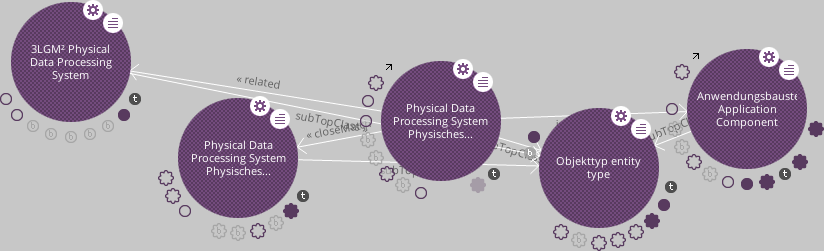
\includegraphics[width=\textwidth]{img/lodlive.png}\\
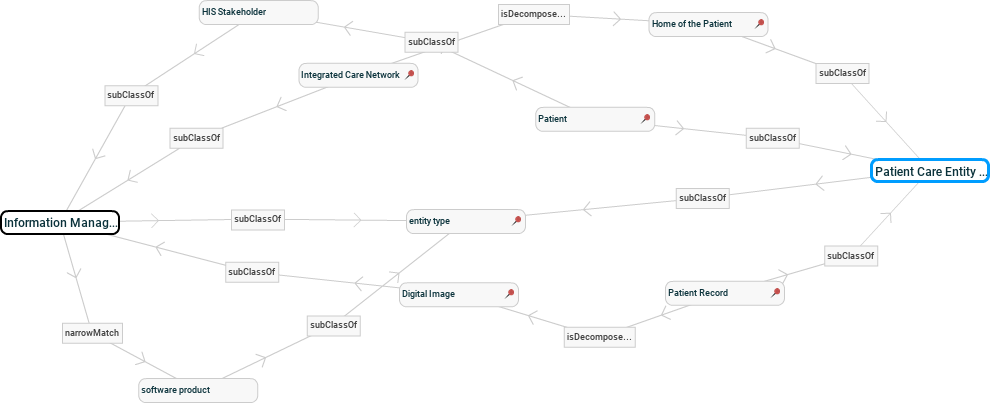
\includegraphics[width=\textwidth]{img/relfinder.png}
\note{
\begin{itemize}
\item über SPARQL Endpunkt kann man auch externe Services anbinden 
\item keinerlei Entwicklungsaufwand für uns
\item Beispiel: LodLive zum schrittweise Graph-Explorieren
\item Beispiel: Relfinder für alle kurzen Wege zwischen zwei Knoten, genaue Beziehung zwischen ihnen
\end{itemize}
}
\end{frame}



\imageslide[https://imise.github.io/snik-ontology/2017/04/12/dashboard]{Statistiken}{img/dashboard-medley.png}{
\begin{itemize}
\item Qualitätsmetriken und Statistiken
\item JavaScript-Bibliothek Sgvizler: SPARQL Queries als Diagramme anzeigen
\end{itemize}
}

\imageslide[\url{http://www.snik.eu/evaluation}]{TripleCheckMate}{img/triplecheckmate.png}{
Stichprobenartige Evaluation einzelner Ressourcen
}

\imageslide[https://github.com/IMISE]{Öffentliche Softwarerepositories}{img/github.png}{
\begin{itemize}
\item Bereitstellung der Software und der Ontologie
\item Ticketsystem 
\end{itemize}
}

\fi

\begin{frame}{Future Work}
\begin{itemize}
\item ontology assisted textbook creation
\item editing in SNIK graph
\item align meta model with General Formal Ontology  
\item ontology matching
\item reasoning
\end{itemize}
\end{frame}


\begin{frame}[fragile]{Fragen?}
\begin{itemize}
%\item Diese Präsentation \url{https://github.com/KonradHoeffner/latex/releases/download/colloquium/colloquium.pdf}
\vspace{0.5em}%here it works as intended
\item Überblick \url{http://www.snik.eu}
\item Visualisierung \url{http://www.snik.eu/graph}
\item SPARQL Endpunkt \url{http://www.snik.eu/sparql}
\item RDF Browser \url{http://www.snik.eu/ontology}
\item Evaluation \url{http://www.snik.eu/evaluation}
\item Twitter \url{https://twitter.com/snik\_proj}
\item Technisches Blog \url{https://imise.github.io/snik-ontology}
\item GitHub Organisation mit Ticketsystem \url{https://github.com/imise}
\end{itemize}
\end{frame}

\end{document}
